\documentclass[smallextended]{svjour3} 
 \usepackage[T1]{fontenc}
\usepackage[utf8]{inputenc}
%\usepackage{fixltx2e}
\usepackage{ifthen,figlatex}
\usepackage{longtable}
\usepackage{float}
\usepackage{wrapfig}
\usepackage{subfigure}
\usepackage{graphicx}
\usepackage[export]{adjustbox}
\usepackage{xspace}
\usepackage{amsmath,amssymb}
\usepackage[french, frenchb]{babel}
\AtBeginDocument{
\definecolor{pdfurlcolor}{rgb}{0,0,0.6}
\definecolor{pdfcitecolor}{rgb}{0,0.6,0}
\definecolor{pdflinkcolor}{rgb}{0.6,0,0}
\definecolor{light}{gray}{.85}
\definecolor{vlight}{gray}{.95}
}
%\usepackage[paper=letterpaper,margin=1.61in]{geometry}
\usepackage{url} \urlstyle{sf}
\usepackage[normalem]{ulem}
\usepackage{todonotes}
\usepackage[colorlinks=true,citecolor=pdfcitecolor,urlcolor=pdfurlcolor,linkcolor=pdflinkcolor,pdfborder={0 0 0}]{hyperref}
\usepackage[round-precision=3,round-mode=figures,scientific-notation=true]{siunitx}
% \usepackage{minted}
% \usepackage{verbments}
% \usepackage{verbatim}
% \usepackage{alltt}

  \usepackage{graphicx}
  \usepackage{hyperref}
\date{\today}
\title{}
\hypersetup{
  pdfkeywords={},
  pdfsubject={},
  pdfcreator={}}
\begin{document}

\newcommand{\AL}[2][inline]{\todo[color=green!50,#1]{\sf \textbf{AL:} #2}\xspace}
\newcommand{\LS}[2][inline]{\todo[color=green!50,#1]{\sf \textbf{LS:} #2}\xspace}

\let\oldcite=\cite
\renewcommand\cite[2][]{~\ifthenelse{\equal{#1}{}}{\oldcite{#2}}{\oldcite[#1]{#2}}\xspace}
\let\oldref=\ref
\def\ref#1{~\oldref{#1}\xspace}
\def\ie{i.e.,\xspace}
\def\eg{e.g.,\xspace}
\def\qrmspu{\texttt{QRM\_StarPU}\xspace}
\sloppy

\title{Simulation d'applications dynamiques pour plateformes de
calculs hautes performances%\thanks{Grants or other notes
%about the article that should go on the front page should be
%placed here. General acknowledgments should be placed at the end of the article.}
}
%\subtitle{Do you have a subtitle?\\ If so, write it here}

\titlerunning{StarPU SMPI}        % if too long for running head

\author{Steven QUINITO MASNADA  \\ \\
        Encadrants : Arnaud LEGRAND \and Luka STANISIC  %if many names separate them with \and.
}

\authorrunning{Steven QUINITO MASNADA} % if too long for running head

\institute{%F. Author \at
           %   first address \\
           %   Tel.: +123-45-678910\\
           %   Fax: +123-45-678910\\
           %   \email{fauthor@example.com}           %  \\
%             \emph{Present address:} of F. Author  %  if needed
           %\and
           %S. Author \at
           %   second address
}

\date{Juin 2015}
% The correct dates will be entered by the editor

\maketitle


\begin{abstract}
Actuellement, la majorité des supercalcultateurs sont des noeuds
composés de machines hybrides. Pour tirer partie de toute la
puissance de calcul disponible, il est indispensable d'avoir un
programme qui soit dynamique. Cependant, les APIs de programmation
classiques conduisent à une mise en oeuvre très complexe.
Le paradigme de programmation par tâches couplé à un système
dynamique permet de répondre à ce problème, mais il est difficile
d'en évaluer les performances. L'objectif de notre étude est donc de
mettre en place les dispositifs nécessaire à l'évaluation de
performances d'un tel système. 
\newpage
\end{abstract}

\section{Introduction}
\label{sec-1}

La majorité des supercalculateurs actuels, comme le montre le site
top500\footnote{http://www.top500.org} sont des clusters
massivement parallèles et composés de noeuds hybrides
(CPU-GPU). Pour les programmer, il existe certains standards. Il y a
tout d'abord la norme MPI (Message Passing Interface), qui est une
API de communication basée sur l'envoi et la réception de
message. Elle a pour objectif d'être performante et portable.  Elle
est de plus haut niveau que les sockets et apporte des mécanismes
comme des fonctions de communications collectives (exemple
broadcast). Ensuite, il y a l'API OpenMP qui est une interface de
multihreading de plus haut niveau de PThread. Elle permet de
découper facilement des traitements et d'exploiter les architectures
multicoeurs. Enfin, il y a l'API CUDA qui permet de tirer partie de
la puissance de calcul des GPUs. Pour cela il est nécessaire de
spécifier explicitement ce que l'on veut envoyer aux GPUs et on doit
également gérer la synchronisation entre les CPUs et les GPUs. 

Si l'on veut optimiser le rendement d'une application afin que
celle-ci tire partie de toute la puissance de calcul disponible, il
est nécessaire d'utiliser plusieurs paradigmes à la fois ce qui
complique grandement la tâches. Nous sommes donc face à un problème 
de programmation classique où l'on doit, avec les APIs précédentes,
indiquer explicitement où et quand chacun des calculs doit être 
réalisé. Par exemple pour exploiter efficacement un GPU, on doit
transférer explicitement les données du CPU vers le GPU, lancer
l'exécution du calcul sur le GPU, gérer la synchronisation sur
l'attente du résultat, récupérer le résultat et pendant ce temps
continuer à occuper le CPU avec un autre calcul. Cet exemple
n'illustre que la difficulté liée à la répartition de charge au
niveau d'un seul et même noeud. Cela se complique davantage lorsque
l'on veut également répartir la charge entre plusieurs machines. 
Cependant même si l'on arrive à équilibrer les charges correctement,
cette solution est difficilement portable vers une autre machine.  

La solution serait donc d'avoir une gestion dynamique des
charges. Mais cela s'avère bien plus compliqué, voir impossible
à réaliser directement avec ces méthodes de
programmation. L'alternative est la programmation par tâches. Ce     
paradigme fournit une abstraction à la notion d'exécution de calculs sur CPU,
GPU et sur d'autres machines. Ainsi le développeur n'a plus à se
soucier de sur quelle ressource le calcul est effectué, mais
seulement d'exprimer le calcul sous la forme d'un graphe de
tâches. De plus avec un système de répartition dynamique
l'utilisateur n'aurait également plus de besoin de soucier de quand
les traitements doivent être effectués. La librairie
StarPU\cite{StarPU} est un exemple utilisant cette approche, c'est
cette dernière que nous allons utiliser. C'est un système runtime
qui permet une répartition des traitements de manière dynamique et
opportuniste. Pour ce faire, StarPU tient à jour un graphe de dépendance
permettant d'optimiser l'ordonnancement des tâches. La première
version de StarPU a été conçu spécialement pour des architectures
hybrides. Une version récente (StarPU MPI)\cite{StarPU-MPI} a été 
réalisée pour bénéficier d'un ordonnancement et d'une exécution qui
soit à la fois dynamique et opportuniste dans un contexte distribuée.

Les performances d'un tel système sont difficiles à évaluer pour
plusieurs raisons. Tout d'abord, la configuration du runtime
est un paramètre à prendre en compte, on peut choisir des
heuristiques et des politiques d'ordonnancements différentes.
Ensuite, il y a les réglages au niveau de l'application qu'il faut
prendre en compte, notamment le découpage des tâches, qui entraîne
la génération d'un graphe de tâches différent.

Dans cet objectif, la première partie de ce rapport montre qu'une
des approches possible est la simulation. La seconde partie
présente en détail le fonctionnement de StarPU et SimGrid 
ainsi que les difficultés rencontrées. La troisième partie est
consacrée à la méthodologie employée.  Une quatrième partie montre la
contribution à la simulation de telles applications.  Et la
cinquième partie aborde ce que nous avons réussit à mettre en place. 

\section{État de l'art}
\label{sec-2}
En HPC, il y a deux grandes approches possibles pour évaluer les
performances d'applications.
\subsection{Test sur systèmes réels}
\label{sec-2-1}
Cette approche consiste à lancer la vrai application sur le système
réel afin d'effectuer les mesures. Cependant cette méthode peut se 
révéler très coûteuse et il n'est pas toujours possible d'avoir
accès à la plateforme. De plus comme les exécutions sont non
déterministes il est indispensable de réaliser un grand nombre
d'expériences, or à cause du coût il n'est possible d'effectuer
qu'un petit nombre de mesures sur un nombre restreint de
plate-formes. Il est donc difficile d'extrapoler ce qui serait
pourtant très utile aux développeurs de runtimes et d'applications. 
\subsection{Simulation}
\label{sec-2-2}
La simulation a pour but de définir un modèle et de calculer une
prédiction du comportement du système avec généralement un code
déterministe et séquentiel. Cela permet ainsi de s'affranchir de la
plateforme et les expériences peuvent être effectuées à partir de
n'importe quel système. Il n'est plus nécessaire d'avoir accès à la
plateforme, ce qui rend cette approche peu coûteuse. Comme la 
simulation nous permettrait d'avoir un contrôle sur de nombreux
paramètres, nous pouvons avoir un système déterministe qui 
nous permettrait d'avoir des expériences qui peuvent être reproduites. 
Par ailleurs il est facile d'extrapoler les résultats car on peut
changer les paramètres du modèle. Enfin la simulation
permet d'avoir un temps d'exécution plus court qu'avec des tests
réels car on n'effectue que certains traitements ce qui nous permet
pouvoir effectuer un grand nombre de mesures.  
\subsubsection{Approche par rejeu de trace}
\label{sec-2-2-1}
Cette méthode consiste à exécuter une première fois l'application
sur un système réel pour ensuite pour ensuite rejouer la trace
post-mortem. Elle est couramment employée dans le contexte 
d'applications MPI statiques. Ici, nous avons à faire à une
exécution complètement dynamique, ce qui est totalement inadaptés car
le flot de contrôle du programme est non déterministes. 
\subsubsection{Approche hybride par simulation / émulation}
\label{sec-2-2-2}
Pour avoir des simulations qui soient réalistes, nous avons besoin
d'exécuter le vrai code et de ne simuler que les communications et
les calculs coûteux. Dans notre cas on simulerait donc la
plateforme de même que l'OS. Et en plus on utiliserait l'émulation
où l'on exécuterait en vrai, mais de manière contrôlée le
programme sur le système simulé. Cette approche est suivie dans
\cite{StarPUSG} où StarPU a été porté sur SimGrid mais avec un
noeud seulement. Notre objectif est d'utiliser la même approche
mais avec plusieurs noeuds et avec StarPU MPI. 

L'approche simulation et émulation se révèle donc la plus adaptée.
Nous avons choisi le simulateur SimGrid qui permet de simuler des
systèmes distribués, des grilles des calculs, des systèmes peer to
peer et cloud. 
\section{Analyse du problème}
\label{sec-3}
\subsection{SimGrid}
\label{sec-3-1}
\begin{figure}[tbh]
\centering
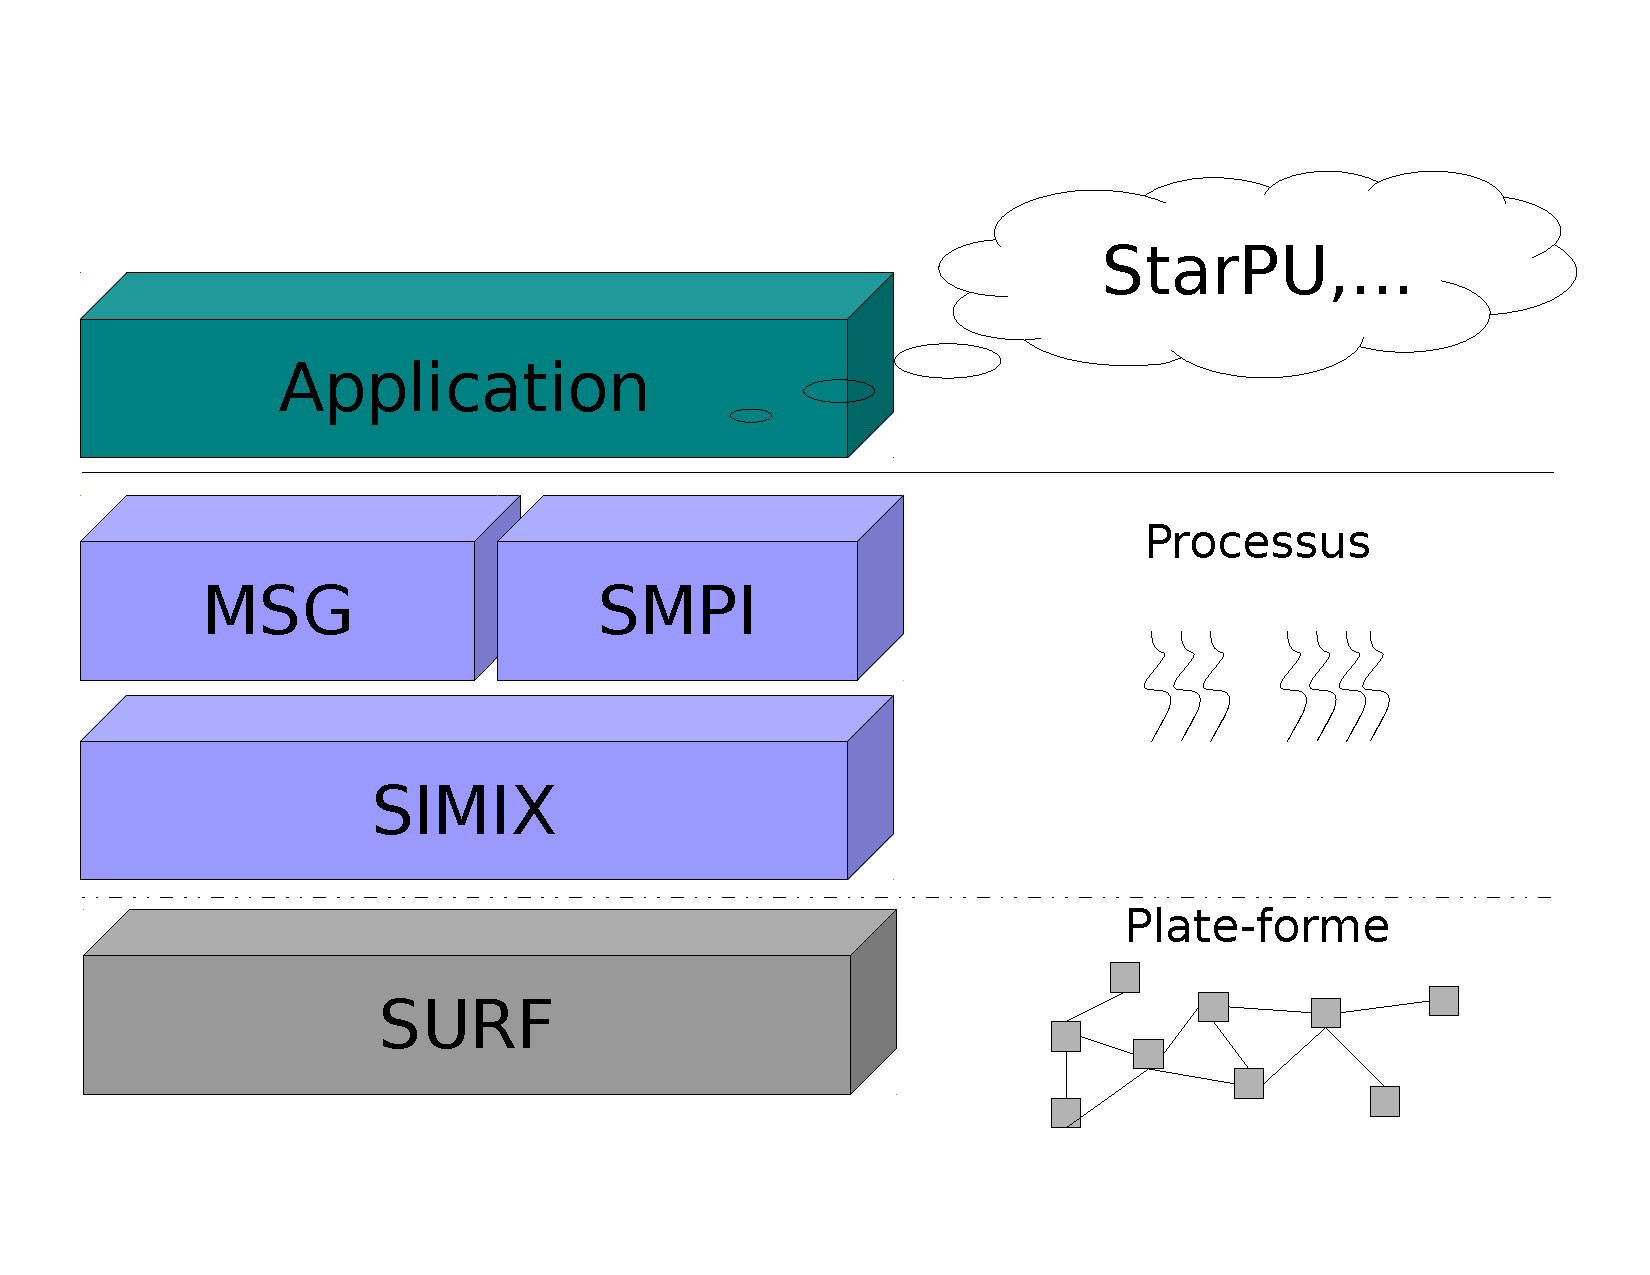
\includegraphics[width=.8\linewidth]{./Img/Simgrid.pdf}
\caption{\label{fig:1}Structure de Simgrid}
\end{figure}

SimGrid est propose de plusieurs APIs et est composé de plusieurs
modules (voir figure\ref{fig:1}). Il y a tout d'abord l'API SURF qui a pour objectif de
décrire les caractéristiques de la plateforme et de la simuler. On
lui fournit donc une modèle de performance qui permettra d'estimer
la durée des calculs et des transferts.

Ensuite, le module SIMIX permet de simuler la partie OS. C'est lui
qui s'occupe notamment de la gestion et de l'ordonnancement des
processus et également des mécanismes de synchronisation. Sous
SimGrid, les processus sont modélisés par des threads, ce qui
signifie que leur espace d'adressage est partagé et nous permet
de simuler un environnement à mémoire partagée facilement. 

Ensuite, au dessus SIMIX, il y a d'une part l'API MSG. Cette dernière
permet à l'utilisateur créer et manipuler des processus de manière
simple. C'est cette API qui est généralement utilisé pour la
plupart des applications classiques et hybrides. 

Et d'autre part, il y a l'API SMPI qui a été développée
spécifiquement pour simuler des applications MPI. Actuellement la
majeure partie des fonctionnalités de MPI ont été implémentées. La
simulation de code MPI est assez compliquée et SimGrid est un des
seul simulateurs à le permettre. 
\begin{figure}[htb]
  \centering
  \begin{minipage}{.45\linewidth}
    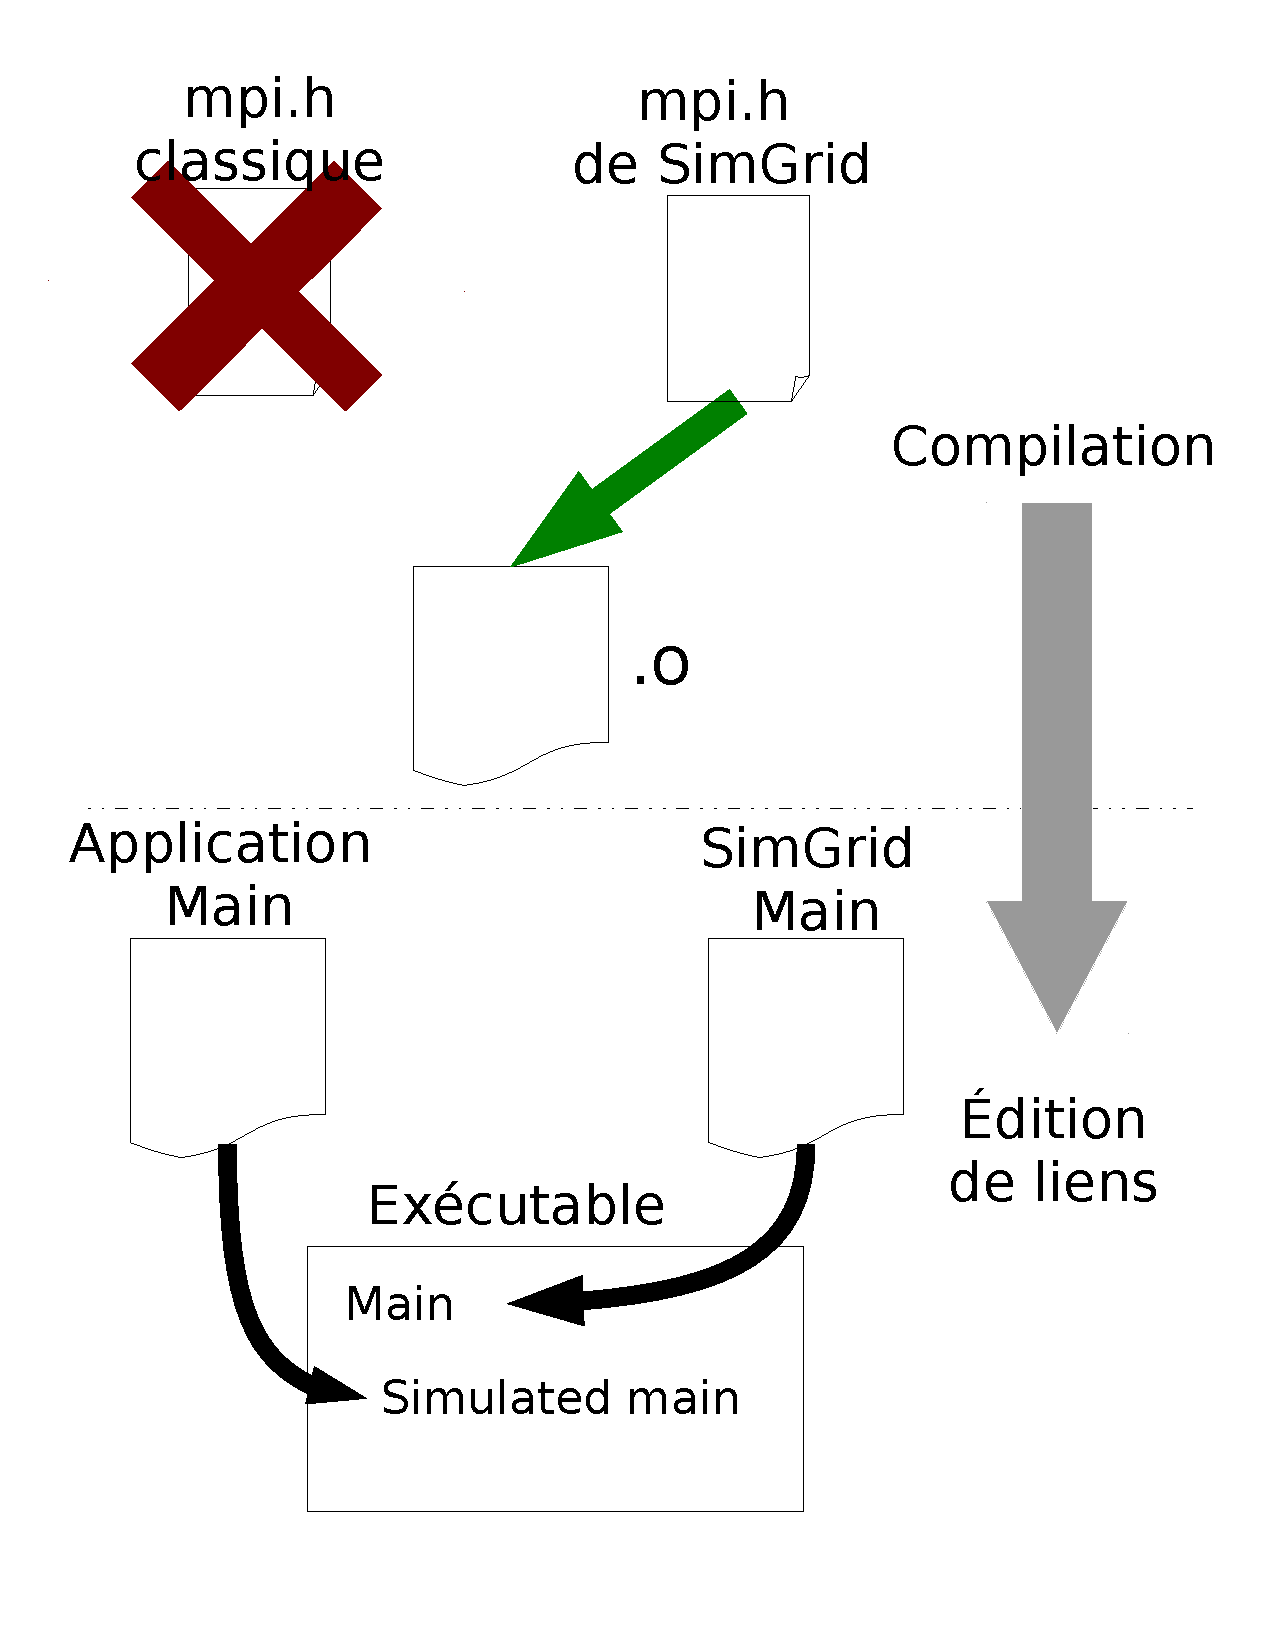
\includegraphics[width=\linewidth]{./Img/Compile.pdf}
    \caption{\label{fig:2}Construction de l'application simulée}
  \end{minipage}
  \begin{minipage}{.45\linewidth}
    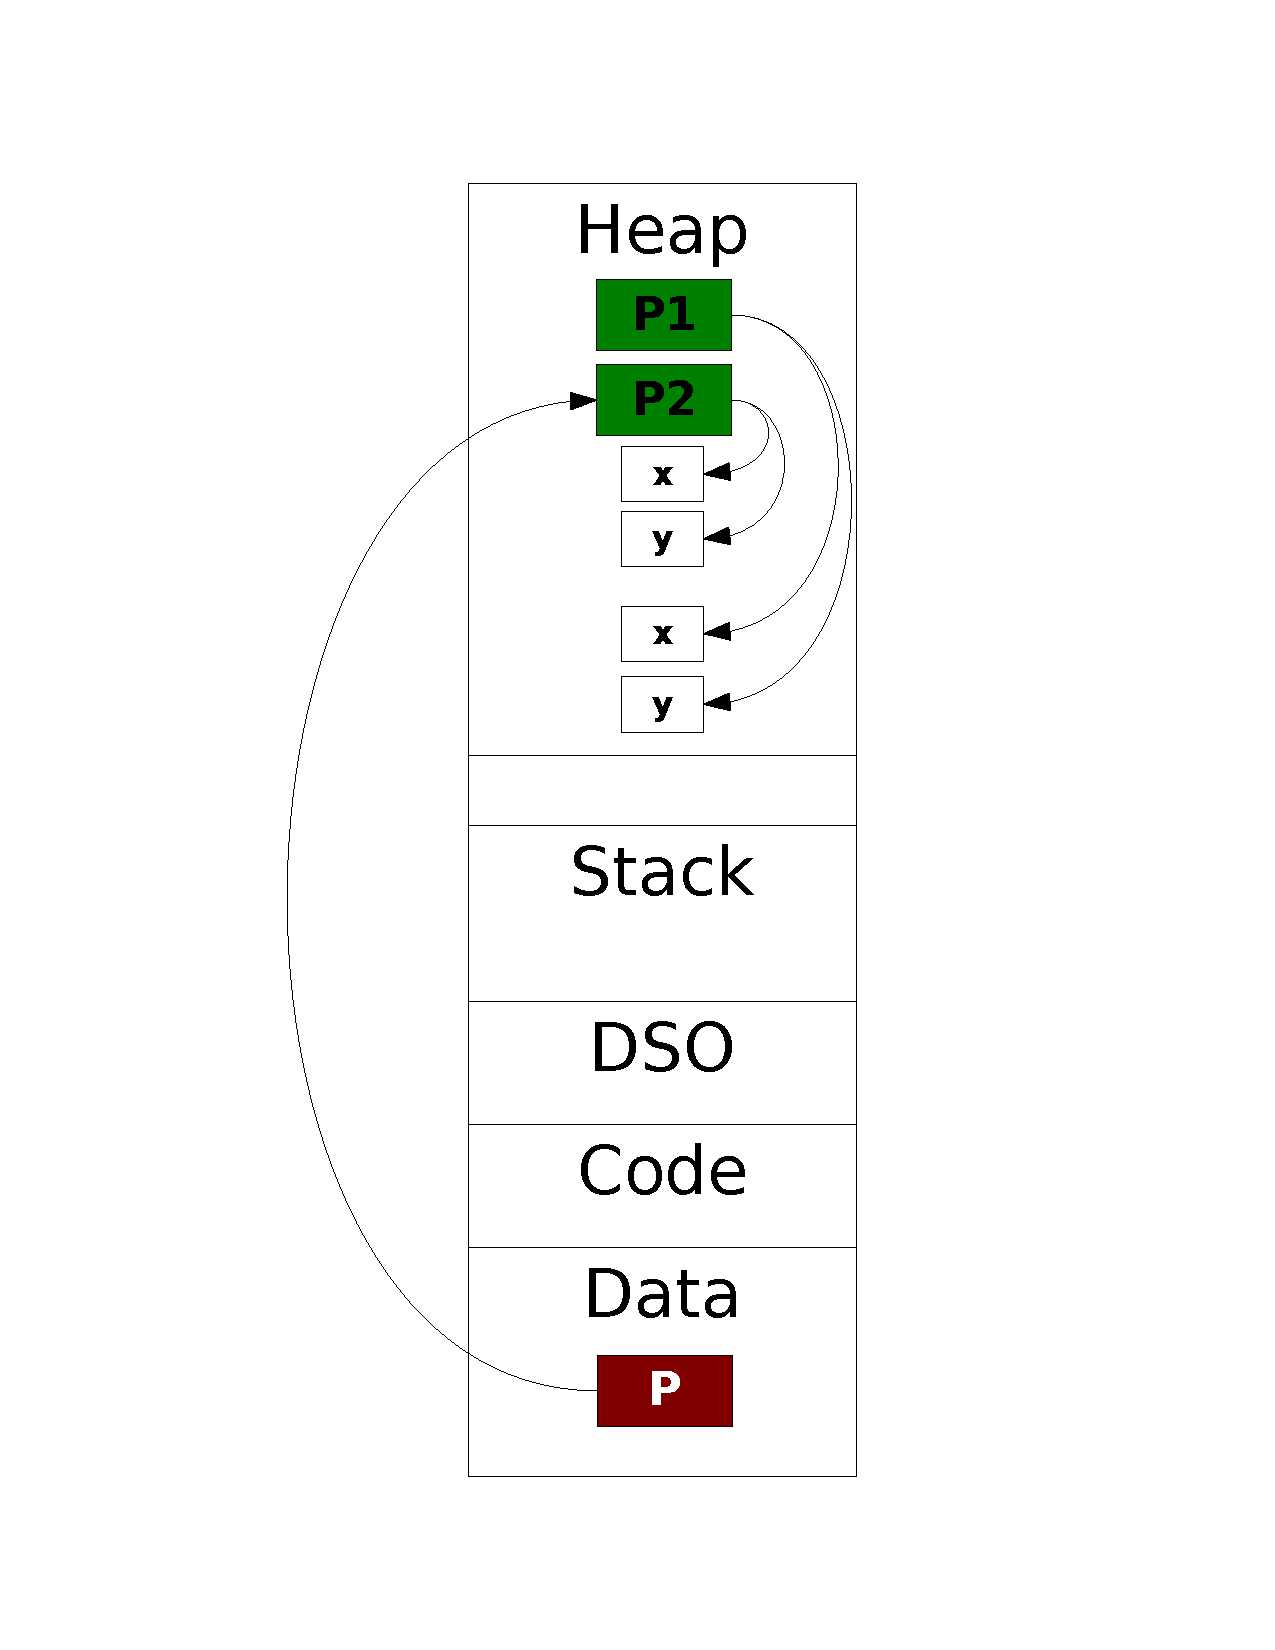
\includegraphics[width=\linewidth]{./Img/Memoire.pdf}
    \caption{\label{fig:3}Privatisation du segment de données}
  \end{minipage}
\end{figure}

Pour ce faire, on compile l'application que l'on veut tester en
remplaçant le mpi.h classique par le mpi.h de SimGrid (voir
figure\ref{fig:2}). Ensuite, à l'édition de liens on remplace 
le main de l'application par le main de SimGrid. Ce dernier a pour
rôle de préparer l'exécution du simulateur en créant la plateforme
et en déployant les processus SMPI qui exécuterons chacun le main
de l'application MPI. Comme dans le cadre d'applications MPI on est
dans un environnement à mémoire distribuée et que sous SimGrid les
processus sont modélisés par des threads, afin de simuler le fait
que chacun ait un espace d'adresse séparé, l'approche suivi par SMPI
consiste à privatiser les variables des processus en créant pour
chacun un segment de données virtuel (voir figure\ref{fig:3}). Pour
cela, pour chaque processus une nouvelle zone mémoire est créée
dans le tas grâce à un mmap, puis le segment de données est recopié
dans cette zone et à chaque changement de contexte on fait pointer
vers la zone correspondant à celle du processus. 

\subsection{StarPU-MSG: Architecture générale}
\label{sec-3-2}
Comme à la base StarPU visait le modèle CPUs-GPUs, l'API la plus
proche était MSG, notamment car le modèle de performances des
communications entre noeuds est différents de celui entre CPUs et
GPUs. StarPU a donc été modifié pour pouvoir fonctionner au dessus
du simulateur SimGrid en se basant sur MSG. Ainsi, l'application
(le runtime de StarPU) est réellement exécutée, mais les
allocations mémoires des tâches ne sont pas effectuées, les codes
de calcul sont simulés et remplacés par un délais de même pour les
transferts CUDA.  

\subsection{StarPU-SMPI:Ce qui coince}
\label{sec-3-3}

\begin{wrapfigure}{r}{40mm}
\vspace{-15mm}
\begin{center}
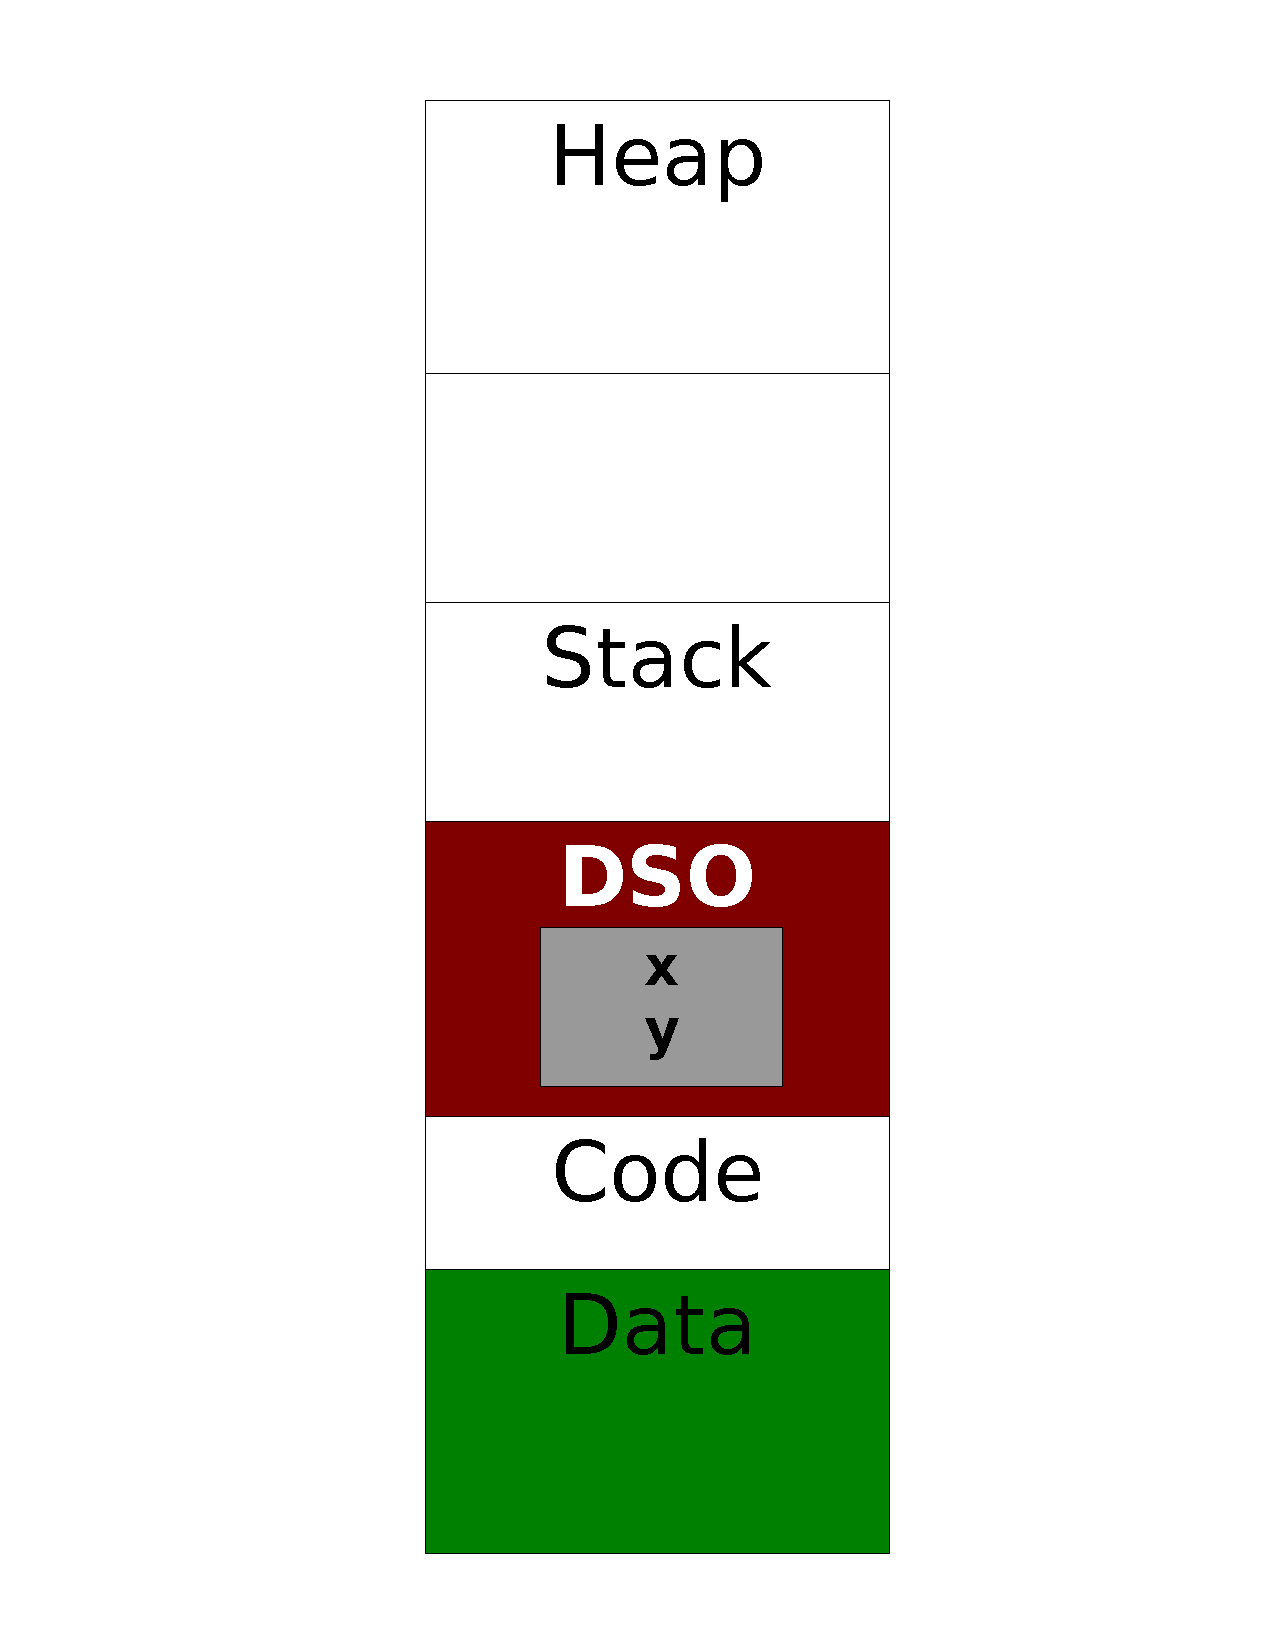
\includegraphics[width=5cm]{./Img/Dyn.pdf}
\end{center}
\caption{\label{fig:4}Emplacement en mémoire des bibliothèques dynamiques}
\end{wrapfigure}

Avec StarPU MPI, la modélisation est différente. On est à la fois
un environnement à mémoire partagée (entre les CPUs et les GPUs
d'une même machine) et un environnement à mémoire distribuée
(entre les différents nœuds). On doit donc permettre d'avoir des
modèles de performances différents selon qu'on est entre noeud où à
l'intérieur d'un nœud. Il nous faut également activer la
privatisation de variables entre les noeuds mais également
permettre le partage de variables à l'intérieur de chacun noeuds. 

Pour cela nous avons besoin de faire fonctionner MSG et SMPI
ensemble. Or non seulement StarPU est essentiellement basé sur MSG
mais MSG et SMPI n'ont par ailleurs pas été prévu pour fonctionner
ensemble même si dans le principe rien ne l'interdit. Il
faudra donc initialiser correctement à la fois la partie MSG et la
partie SMPI.  

Il y a un également un autre point à prendre en considération,
celui des librairies dynamiques. 

Dans SimGrid seul le segment données est privatisé, comme les
variables globales des librairies dynamiques ne se trouvent pas
dans ce dernier (DSO sur la figure\ref{fig:4}), elles restent donc
accessible accessibles à tous les processus SimGrid. Nous devrons donc
également faire en sorte de privatiser les variables globales des
librairies externes entre les noeuds. 

\section{Méthodologie}
\label{sec-4}
Comme nous travaillons avec SimGrid et StarPU à la fois, nous
utilisons un dépôt complexe comprenant les deux et géré avec
l'outils submodule de \href{https://github.com/swhatelse/Journal}{git}. Ce dernier nous permet de gérer des sous
dépôt indépendemment, ainsi il est plus aisé de traiter les mises à
jours de ces derniers.

Afin de pouvoir retracer le cheminement de mon travail, mais aussi
de pouvoir garder le fil d'un jour à l'autre, un cahier de
laboratoire est tenu en org-mode et est hébergé sur github.

Comme on l'a vu précédemment il est nécessaire d'apporter quelques
modifications au niveau du simulateur et de StarPU. Dans ce but, il
a été dans un premier temps nécessaire de consulter la documentation
afin de comprendre le fonctionnement et l'architecture de
SimGrid. Ensuite il a fallut explorer le code afin de déterminer où
et comment apporter les modifications. Pour cela les outils tels que
GDB et Valgrind ont été d'une aide précieuse et ont permis de notamment
vérifier que les changements de segment mémoire s'effectuent bien au
bon moment.

\section{Contribution}
\label{sec-5}
La toute première chose à réaliser, a été la gestion du partage du
segment de données au niveau du simulateur dans un contexte
SMPI. Comme la mémoire est partagée au sein d'un noeud, nous avons
fait en sorte que les processus d'un même noeud aient leurs segment
données en commun. Le principe est le suivant, il y a dans un
premier temps, les processus SMPI qui sont créés au lancement de
l'application avec leur propre espace de données. Puis ces derniers
peuvent à leurs tours créer de nouveau processus. Ceux-ci héritent
donc du segment de données du processus qui les a créés. Il a par
ailleurs été nécessaire d'initialiser MSG et SMPI
correctement afin que les deux puissent fonctionner
ensemble. SimGrid a donc été modifié en conséquences. 

\begin{wrapfigure}{r}{40mm}
\begin{center}
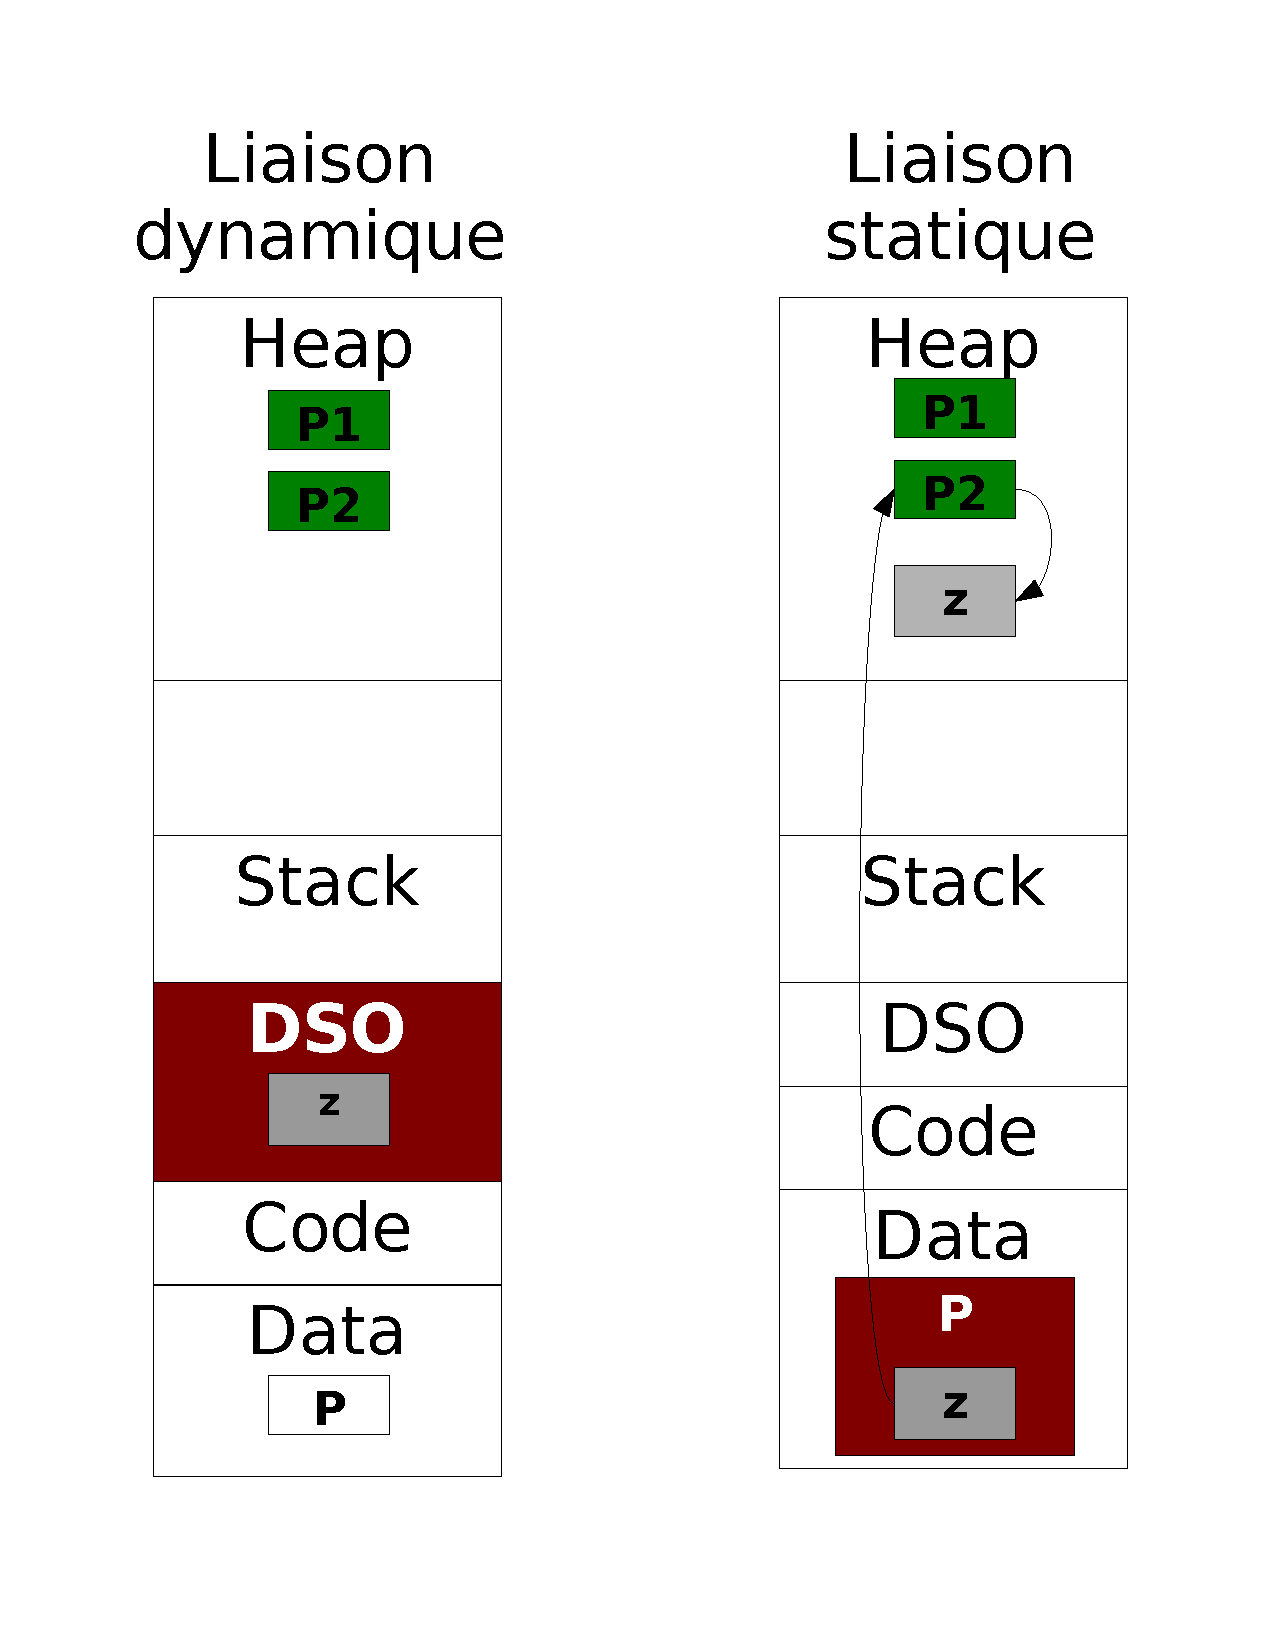
\includegraphics[width=5cm]{./Img/StaticDyn.pdf}
\end{center}
\caption{\label{fig:5}Emplacement en mémoire des bibliothèques}
\end{wrapfigure}

Une fois la gestion du partage mise en place, nous nous sommes
penchés sur le cas des bibliothèques dynamiques. Nous avons vu
précédemment que malgré le mécanisme de privatisation, les variables
globales présentes dans ces dernières sont partagés entre les
différents processus SimGrid. Pour contourner ce problème, nous
avons décidé d'utiliser une version statique de la bibliothèque.  

Ainsi avec une bibliothèque statique, les variables globales de
celle-ci se retrouvent dans le segment données du processus et la
gestion du partage / privatisation est géré par le mécanisme
précédent (voir figure\ref{fig:5}) . Cette solution est relativement intrusive car
elle nécessite de changer la chaîne de compilation des applications
utilisant StarPU, mais cela sera suffisants dans un premier temps. 

Comme StarPU a été porté au dessus de MSG, il a également été
nécessaire d'apporter quelques modifications au niveau de
l'initialisation. Car le mécanisme de gestion de la privatisation et
de partage n'était activée que de manière tardive. 

\section{Validation}
\label{sec-6}
\subsection{Test simple}
\label{sec-6-1}
Dans le but de tester le bon fonctionnement des modifications
apportées, un test illustrant le fonctionnement de StarPU a été
fourni et enrichi. Ce dernier permet ainsi d'isoler le problème
afin de pouvoir nous concentrer dessus. Ce test, initialise SimGrid
et la partie SMPI comme cela est fait du côté de StarPU et fait
appel à une bibliothèque dynamique et manipule des variables
globales. Ainsi lors de l'exécution de ce test, on doit pouvoir
constater que pour des processus appartenant à un même noeuds, les
valeurs des variables globales du programme et des bibliothèques
dynamiques sont bien identiques.  
\subsection{Test de StarPU - SMPI}
\label{sec-6-2}
Comme les résultats du test simples étaient ceux attendu, nous
sommes passé à un test utilisant cette fois la vrai bibliothèque
StarPU. Cette dernière est fourni avec des exemples de programme MPI
notamment d'algèbre linéaire tel que l'algorithme de Cholesky. Nous
nous sommes servi de ces derniers afin de valider les
modifications. 
\section{Conclusion}
\label{sec-7}
Pour conclure, nous avons apporté les modifications nécessaire à 
SimGrid et StarPU afin de pouvoir simuler des applications MPI basées 
sur StarPU MPI. La difficulté résidait dans le fait de comprendre des 
programmes complexes avec de nombreuses lignes de codes (106350 lignes 
pour Simgrid et 172251 lignes pour StarPU) et d'arriver à repérer où 
effectuer les modifications tout en faisant en sorte qu'elles soient 
minimes (ici une vingtaine de lignes ont été ajoutées à SimGrid et
StarPU). 

La prochaine étape sera d'effectuer les simulations et les mesures. 
Pour ce faire les expériences seront faites avec un solveur d'algèbre 
linéaire basé sur StarPU. Dans le but de valider le résultat des 
expérimentations, un test grandeur nature sera fait sur Grid5000.  

\section*{Acknowledgments}
Je souhaite remercier Bruno GAUJAL pour m'avoir permis de faire mon
stage dans son équipe. Ensuite, je souhaite  remercier
Arnaud LEGRAND, mon tuteur de stage pour avoir été
aussi disponible et pour sa patience, pour avoir su me guider tout
au long de ce TER, et également pour m'avoir tellement appris. Grâce
à cela j'ai trouvé un domaine qui me plaît particulièrement. Je souhaite
également remercier Luka STANISIC pour m'avoir aidé lorsque je
bloquais et donné des astuces très utiles. Et je remercie également
Thibaud BUCHS pour ces pauses cafés et pour son aide également. 
\nocite{*}
\def\raggedright{}
\bibliographystyle{IEEEtran}
\bibliography{biblio}
\end{document}